\input{header}

\AtBeginSubsection[]
{
	\begin{frame}<beamer>
		\frametitle{Outline}
		\tableofcontents[current,currentsubsection]
	\end{frame}
}

\begin{document}

\begin{frame}[allowframebreaks] \frametitle{Undecidable problems}
  \begin{itemize}
\item There quite a few undecidable problems

\item For example, program verification is in general not solvable

\item We will discuss an undecidable example called the ``halting problem''
  
\end{itemize}\end{frame} \begin{frame}[allowframebreaks] \frametitle{$A_{TM}$}
\begin{equation*}
  A_{TM}=\{
\langle  M,w\rangle \mid M: \mbox{ a TM that accepts } w\}
\end{equation*}
  \begin{itemize}
\item We will prove that $A_{TM}$ is undecidable
\item However, $A_{TM}$ is Turing recognizable

\item We can simply simulate $\langle  M,w\rangle $
\item To be decidable we hope to avoid an infinite loop

\item [] if at one point, know it cannot halt

$\Rightarrow$ reject
\item Thus this problem is called the halting problem
\end{itemize}\end{frame} \begin{frame}[allowframebreaks] \frametitle{Diagonalization method}
  \begin{itemize}
\item We need a technique called ``diagonalization method'' for the proof
\item It was developed by Cantor  in 1873
to check if two  infinite sets are equal

\item Example: consider
  \begin{center}
  set of even integers
\end{center}
versus
\begin{center}
set of $\{0,1\}^*$
\end{center}
\item Both are infinite sets. Which one is larger ?
\item Definition: two sets are equal if elements
can be paired
\end{itemize}\end{frame} \begin{frame}[allowframebreaks] \frametitle{Definition 4.12}
  \begin{itemize}
\item $f$ is a one-to-one function if:
  \begin{equation*}
f(a)\neq f(b) \text{ if } a \neq b
\end{equation*}

\begin{center}
  \begin{tabular}{cc}
\begin{tikzpicture}
  \draw[->] (-1.5, 0) -- (1.5, 0) node[right] {$x$};
  \draw[->] (0, -0.5) -- (0, 2.2) node[above] {$y$};
  \draw[-][scale=0.5, domain=-2.2:2.2, smooth, variable=\x, blue] plot ({\x}, {0.5*exp(\x)});
\end{tikzpicture}
    &
\begin{tikzpicture}
  \draw[->] (-1.5, 0) -- (1.5, 0) node[right] {$x$};
  \draw[->] (0, -0.5) -- (0, 2.2) node[above] {$y$};
  \draw[-][scale=0.5, domain=-2:2, smooth, variable=\x, blue] plot ({\x}, {\x*\x});
\end{tikzpicture}
% \begin{tikzpicture}
%   \draw[->] (-0.5, 0) -- (2.2, 0) node[right] {$x$};
%   \draw[->] (0, -1.3) -- (0, 1.5) node[above] {$y$};
%   \draw[scale=0.5, domain=-2:2, smooth, variable=\y, red]  plot ({\y*\y}, {\y});
% \end{tikzpicture}
  \end{tabular}
\end{center}
\item Left: a one-to-one function; right: not
\item $f:A\rightarrow B$ onto if 
  \begin{equation*}
\forall b \in B, \exists a \text{ such that } f(a)=b
\end{equation*}
\item Example:
  \begin{equation*}
    f(a) = a^2, \text{ where } A = (-\infty, \infty) \text{ and }
    B = (-\infty, \infty)
  \end{equation*}
  This is not an onto function because for $b = -1$, there is no
  $a$ such that $f(a) = b$
\item However, if we change it to
    \begin{equation*}
    f(a) = a^2, \text{ where } A = (-\infty, \infty) \text{ and }
    B = [0, \infty)
  \end{equation*}
it becomes an onto function
\item Definition: a function is called a
  correspondence if it is one-to-one and onto
\item Example:
      \begin{equation*}
    f(a) = a^3, \text{ where } A = (-\infty, \infty) \text{ and }
    B = (-\infty, \infty)
  \end{equation*}
\end{itemize}\end{frame} \begin{frame}[allowframebreaks] \frametitle{Example 4.13}
  \begin{itemize}
\item $N=\{1,2,\ldots\}$
\item $E=\{2,4,\ldots\}$
\item The two sets can be paired
  \begin{center}
    \begin{tabular}{cc}
$n$ & $f(n)=2n$\\ \hline
1 & 2 \\
2 & 4 \\
$\vdots$ & $\vdots$
    \end{tabular}
  \end{center}
\item We consider $N$ and $E$ have \alert{the same size}
\item Definition: a set is countable if it is 
  \begin{center}
finite or same size as $N$
\end{center}
\end{itemize}\end{frame} \begin{frame}[allowframebreaks] \frametitle{Rational Numbers Countable}
  \begin{itemize}
\item $Q=\{m/n
\mid m,n \in N\}$ countable


  \begin{center}
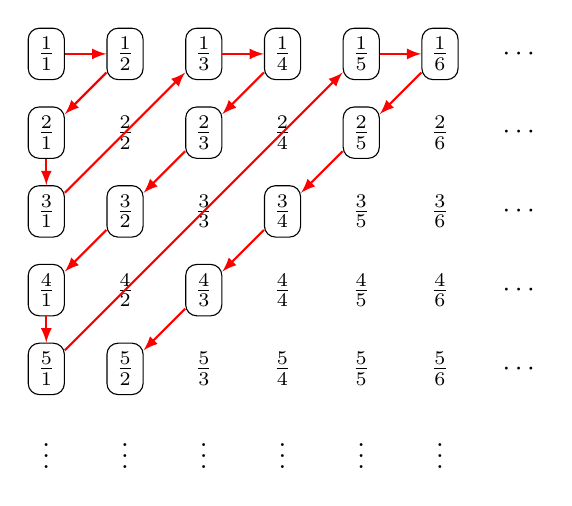
\begin{tikzpicture}
\tikzstyle{keepstyle} =[rectangle, rounded corners, draw, fill=white]
\node at (0,0) {$\vdots$};
\node[keepstyle] (51) at (0,1) {$\frac{5}{1}$};
\node[keepstyle] (41) at (0,2) {$\frac{4}{1}$};
\node[keepstyle] (31) at (0,3) {$\frac{3}{1}$};
\node[keepstyle] (21) at (0,4) {$\frac{2}{1}$};
\node[keepstyle] (11) at (0,5) {$\frac{1}{1}$};
\node at (1,0) {$\vdots$};
\node[keepstyle] (52) at (1,1) {$\frac{5}{2}$};
\node at (1,2) {$\frac{4}{2}$};
\node[keepstyle] (32) at (1,3) {$\frac{3}{2}$};
\node at (1,4) {$\frac{2}{2}$};
\node[keepstyle] (12) at (1,5) {$\frac{1}{2}$};
\node at (2,0) {$\vdots$};
\node at (2,1) {$\frac{5}{3}$};
\node[keepstyle] (43) at (2,2) {$\frac{4}{3}$};
\node at (2,3) {$\frac{3}{3}$};
\node[keepstyle] (23) at (2,4) {$\frac{2}{3}$};
\node[keepstyle] (13) at (2,5) {$\frac{1}{3}$};
\node at (3,0) {$\vdots$};
\node at (3,1) {$\frac{5}{4}$};
\node at (3,2) {$\frac{4}{4}$};
\node[keepstyle] (34) at (3,3) {$\frac{3}{4}$};
\node at (3,4) {$\frac{2}{4}$};
\node[keepstyle] (14) at (3,5) {$\frac{1}{4}$};
\node at (4,0) {$\vdots$};
\node  at (4,1) {$\frac{5}{5}$};
\node at (4,2) {$\frac{4}{5}$};
\node at (4,3) {$\frac{3}{5}$};
\node[keepstyle] (25) at (4,4) {$\frac{2}{5}$};
\node[keepstyle] (15) at (4,5) {$\frac{1}{5}$};
\node at (5,0) {$\vdots$};
\node  at (5,1) {$\frac{5}{6}$};
\node at (5,2) {$\frac{4}{6}$};
\node at (5,3) {$\frac{3}{6}$};
\node at (5,4) {$\frac{2}{6}$};
\node[keepstyle] (16) at (5,5) {$\frac{1}{6}$};
\node at (6,1) {$\cdots$};
\node at (6,2) {$\cdots$};
\node at (6,3) {$\cdots$};
\node at (6,4) {$\cdots$};
\node at (6,5) {$\cdots$};
\draw [-latex,red, thick] (11) -- (12);
\draw [-latex, red, thick] (12) -- (21);
\draw [-latex, red, thick] (21) -- (31);
\draw [-latex, red, thick] (31) -- (13);
\draw [-latex, red, thick] (13) -- (14);
\draw [-latex, red, thick] (14) -- (23);
\draw [-latex, red, thick] (23) -- (32);
\draw [-latex, red, thick] (32) -- (41);
\draw [-latex, red, thick] (41) -- (51);
\draw [-latex, red, thick] (51) -- (15);
\draw [-latex, red, thick] (15) -- (16);
\draw [-latex, red, thick] (16) -- (25);
\draw [-latex, red, thick] (25) -- (34);
\draw [-latex, red, thick] (34) -- (43);
\draw [-latex, red, thick] (43) -- (52);
\end{tikzpicture}
\end{center}

{\small (Latex source from \url{https://divisbyzero.com/2013/04/16/countability-of-the-rationals-drawn-using-tikz/})}

\item Note that we skip counting elements with common factors (e.g., $2/2$)
\end{itemize}\end{frame} \begin{frame}[allowframebreaks] \frametitle{Real Numbers not Countable}
  \begin{itemize}
\item We will use the diagonalization method 
\item The proof is by contradiction
\item Assume $R$ is countable. Then there is a table as follows
  \begin{center}
  \begin{tabular}{r|r}
$n$ & $f(n)$ \\ \hline
1 & 3.14159 $\ldots$\\
2 & 55.55555$\ldots$\\
3 & 0.12345 $\ldots$ \\
4 & 0.50000 $\ldots$ \\
$\vdots$ & 
  \end{tabular}
\end{center}

\item Consider
  \begin{equation*}
    \begin{split}
&    x=0.4641\ldots\\
&    4\neq 1, 6 \neq 5
  \end{split}
\end{equation*}
\item We have
  \begin{equation*}
x \neq f(n), \forall n
\end{equation*}
\item But $x \in R$, so a contradiction
\item To avoid the problem
  \begin{equation*}
  1=0.9999\cdots
\end{equation*}
for every digit of $x$ we should not choose 0 or 9
\end{itemize}\end{frame}


\end{document}

%%% Local Variables:
%%% mode: latex
%%% TeX-master: t
%%% End:
